\documentclass[11pt,a4paper]{article}
\usepackage[margin=2.3cm]{geometry}
\IfFileExists{lmodern.sty}{\usepackage{lmodern}}{}
\usepackage[T1]{fontenc}
\usepackage{titlesec,tabularx,longtable,booktabs,array,enumitem,xcolor,fancyhdr,amsmath}
\usepackage{listings}
\usepackage{tikz}
\usetikzlibrary{arrows.meta,positioning,fit,calc,shapes.geometric,backgrounds}
\usepackage[hyphens]{url}
\usepackage{hyperref}

\definecolor{headcolor}{RGB}{15,70,60}
\definecolor{boxa}{RGB}{226,239,236}
\definecolor{boxb}{RGB}{238,242,250}
\definecolor{boxc}{RGB}{250,243,230}
\definecolor{boxd}{RGB}{245,245,245}
\definecolor{edge}{RGB}{70,70,70}
\hypersetup{colorlinks=true,linkcolor=headcolor,urlcolor=headcolor,
  pdftitle={TrustBazaar System Design - Unit 4: Delivery and Handover},
  pdfauthor={S. M. Nihal Ahmed, Afrim Hossen Khan, Sabikun Nahar Sinthia}}

\titleformat{\section}{\normalfont\Large\bfseries\color{headcolor}}{\thesection}{10pt}{}
\titleformat{\subsection}{\normalfont\large\bfseries}{\thesubsection}{8pt}{}
\titleformat{\subsubsection}{\normalfont\normalsize\bfseries}{\thesubsubsection}{6pt}{}
\pagestyle{fancy}\fancyhf{}
\fancyhead[L]{System Design Document}\fancyhead[R]{Unit 4: Delivery \& Handover}
\fancyfoot[C]{\thepage}\renewcommand{\headrulewidth}{0.4pt}\setlength{\headheight}{14pt}
\setlength{\emergencystretch}{3em}
\setlength{\parskip}{0.45em}\setlength{\parindent}{0pt}

\lstdefinelanguage{SQLpg}{morekeywords={CREATE,TABLE,TYPE,AS,ENUM,PRIMARY,KEY,REFERENCES,NOT,NULL,DEFAULT,CHECK,UNIQUE,INDEX,ON,WHERE,TRIGGER,BEFORE,INSERT,UPDATE,DELETE,FOR,EACH,ROW,EXECUTE,FUNCTION,RETURNS,LANGUAGE,BEGIN,END,IF,THEN,ELSE,RETURN,SELECT,FROM,INTO,ORDER,BY,DESC,LIMIT,GRANT,REVOKE,TO,SCHEMA,EXTENSION,EXISTS,OR,AND,IN,IS,ALTER,ADD,FOREIGN,GENERATED,ALWAYS,IDENTITY,DEFERRABLE,INITIALLY,DEFERRED,DECLARE,PERFORM,LOOP,RAISE,EXCEPTION,USING,DISTINCT,ROLE,LOGIN,USAGE,ALL,TABLES,STABLE,DO},sensitive=false,morecomment=[l]{--},morestring=[b]'}
\lstset{basicstyle=\ttfamily\scriptsize,columns=fullflexible,keepspaces=true,breaklines=true,
  keywordstyle=\color{headcolor}\bfseries,commentstyle=\color{gray}\itshape,frame=single,rulecolor=\color{gray!40},
  upquote=true,literate={–}{{--}}1}

\newenvironment{dtable}[1]{\small\begin{longtable}{#1}}{\end{longtable}}

\begin{document}
\begin{titlepage}
\centering
\vspace*{1cm}
{\Large Daffodil International University}\\[0.2cm]
{\large Department of Software Engineering}\\[2cm]
\rule{\linewidth}{0.5pt}\\[0.4cm]
{\huge\bfseries System Design Document}\\[0.3cm]
{\LARGE Unit 4: Delivery \& Handover}\\[0.3cm]
{\large TrustBazaar: A Verified Peer-to-Peer Auction and Marketplace Platform for Used Goods}\\[0.2cm]
\rule{\linewidth}{0.5pt}\\[1.6cm]
{\large S. M. Nihal Ahmed (232-35-002)\\[0.1cm] Afrim Hossen Khan (232-35-076)\\[0.1cm] Sabikun Nahar Sinthia (232-35-475)}\\[1.6cm]
\begin{tabular}{|l|>{\raggedright\arraybackslash}p{8cm}|}
\hline
\textbf{Status} & Draft for team review \\ \hline
\textbf{Version} & 0.1, 18 October 2026 \\ \hline
\textbf{Implements} & SRS v2.0 (\texttt{docs/srs.tex}) \\ \hline
\textbf{Depends on} & Unit 1 (Identity \& Access), Unit 2 (Order, Payment \& Escrow), Unit 3 (Auctions, Listings \& Search) \\ \hline
\textbf{Database schema} & \texttt{docs/design/sql/04\_delivery.sql}, tested on PostgreSQL (90 checks and concurrency tests, Appendix B) \\ \hline
\end{tabular}
\vfill
\end{titlepage}
\tableofcontents
\newpage
\section{Introduction}

\subsection{Purpose}
This document is the fourth unit of TrustBazaar's System Design Document. It covers how a paid physical item reaches the buyer. There are two ways:
\begin{itemize}[nosep]
  \item \textbf{a meetup handover} at a safe public place, proved by a one-time code that the buyer gives the seller after inspecting the item;
  \item \textbf{courier delivery} at a fare fixed at checkout, tracked through the courier's status updates.
\end{itemize}
The unit records the two facts on which Unit~2's escrow depends: the \emph{fulfilment step} (handover, or courier pickup), whose deadline decides whether the buyer is refunded, and the \emph{delivery event}, from which the dispute window and the auto-release timeout are counted (SRS FR-PAY-07, FR-PAY-08). Acceptance criterion~3 (money is never released before the item is delivered) therefore depends on this unit recording these facts truthfully.

The unit follows conventions DC-1 to DC-13 (Unit~1 Section~2; Unit~2 Section~2.3) and adds DC-14 (Section~\ref{sec:dc14}). Game-account handover is not part of this unit; it is Unit~5.

\subsection{Scope}
\textbf{In scope:}
\begin{itemize}[nosep]
  \item the distance between buyer and seller, the recommended method, and the delivery zones;
  \item courier fares, the versioned fare table, and quotes fixed at checkout;
  \item curated safe meetup points and the suggestion of points near the midpoint;
  \item meetup proposals and agreement, the handover code, the wrong-entry lock and the operator unlock;
  \item courier booking, exact addresses, provider webhooks and status queries, the shipment status machine, failed delivery and return to the seller;
  \item return shipments ordered by a dispute decision (FR-DSP-06(d));
  \item the mock courier and its labelling as simulated;
  \item the fulfilment records used in a dispute case file (FR-DSP-05).
\end{itemize}

\textbf{Out of scope, owned by other units:}
\begin{itemize}[nosep]
  \item escrow state, deadlines, refunds and the split of the delivery fee (Unit~2; this unit reports steps and events through \texttt{EscrowCommands});
  \item the listing's parcel classes, fulfilment options and location (Unit~3, read through its port);
  \item credential handover and takeover for game accounts (Unit~5);
  \item delivering notifications and deadline reminders (Unit~6; this unit emits events);
  \item dispute decisions and the operator queues (Unit~7; this unit supplies the records, the issues and the return booking).
\end{itemize}

\subsection{Requirements covered}
\begin{itemize}[nosep]
  \item \textbf{Functional:} FR-DLV-01 to FR-DLV-14; FR-PAY-08 and FR-PAY-09 (fulfilment side); FR-DSP-01 (when a \texttt{not\_received} dispute may open), FR-DSP-05 (delivery and handover records) and FR-DSP-06(d) (return by courier); FR-NTF-07 (the events behind meetup and pickup reminders); FR-PRV-01 (the courier as a recipient of personal data).
  \item \textbf{Security:} SEC-PAY-03, SEC-PAY-04, SEC-PAY-05 and SEC-PAY-07, applied to the courier; SEC-DAT-07 (the code and addresses never logged); SEC-ACC-05 (masked addresses for staff); SEC-INP-05; SEC-ABU-01.
  \item \textbf{Other:} IF-SW-04, IF-COM-03; NFR-REL-04 (courier outage); NFR-CMP-05 (simulated bookings); DR-06.
\end{itemize}

% ------------------------------------------------------------------
\section{Unit Overview}

\subsection{Responsibilities}
\begin{enumerate}[nosep]
  \item Offer the buyer the methods the seller allows, recommend one by distance, and fix a courier fare at checkout from a published fare table.
  \item Let buyer and seller agree a time at a safe public place without revealing where either of them lives.
  \item Record a meetup handover only when the buyer has released the code, and stop guessing of the code.
  \item Book the courier, keep exact addresses confidential, and turn the courier's status reports into exactly one fulfilment step and one delivery event, however often and in whatever order the reports arrive.
  \item Hand every case that a rule cannot decide (a locked code, a pickup after cancellation, a report that makes no sense) to an operator rather than guessing.
\end{enumerate}

\subsection{Components}
\begin{figure}[!htbp]
\centering
\resizebox{\textwidth}{!}{%
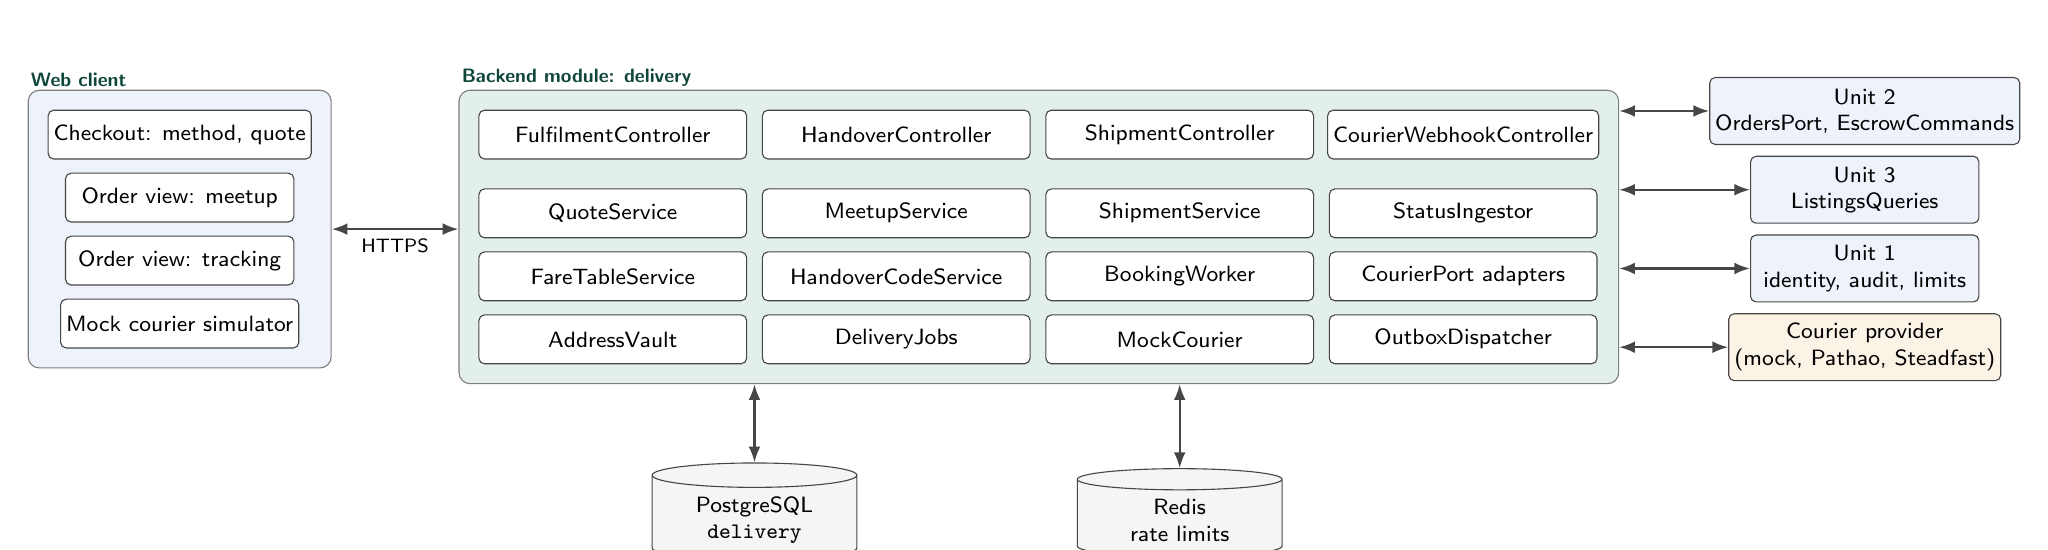
\begin{tikzpicture}[
  font=\sffamily\footnotesize,
  comp/.style={draw=edge, rounded corners=2pt, fill=white, minimum width=2.9cm, minimum height=0.62cm, align=center, inner sep=2pt},
  grp/.style={draw=edge!70, rounded corners=4pt, inner sep=7pt},
  lbl/.style={font=\sffamily\scriptsize\bfseries, text=headcolor, anchor=south west, inner sep=1pt},
  arr/.style={-{Latex[length=2mm]}, draw=edge, thick},
  store/.style={draw=edge, fill=boxd, cylinder, shape border rotate=90, aspect=0.18, minimum width=2.6cm, minimum height=1.1cm, align=center}
]
\node[comp] (c1) at (0,3.9) {Checkout: method, quote};
\node[comp] (c2) at (0,3.1) {Order view: meetup};
\node[comp] (c3) at (0,2.3) {Order view: tracking};
\node[comp] (c4) at (0,1.5) {Mock courier simulator};
\begin{scope}[on background layer]\node[grp, fill=boxb, fit=(c1)(c4)] (client) {};\end{scope}
\node[lbl] at (client.north west) {Web client};
\foreach \n/\x/\y/\t in {k1/5.5/3.9/FulfilmentController, k2/9.1/3.9/HandoverController, k3/12.7/3.9/ShipmentController, k4/16.3/3.9/CourierWebhookController,
  s1/5.5/2.9/QuoteService, s2/9.1/2.9/MeetupService, s3/12.7/2.9/ShipmentService, s4/16.3/2.9/StatusIngestor,
  s5/5.5/2.1/FareTableService, s6/9.1/2.1/HandoverCodeService, s7/12.7/2.1/BookingWorker, s8/16.3/2.1/CourierPort adapters,
  s9/5.5/1.3/AddressVault, s10/9.1/1.3/DeliveryJobs, s11/12.7/1.3/MockCourier, s12/16.3/1.3/OutboxDispatcher}
  {\node[comp, minimum width=3.4cm] (\n) at (\x,\y) {\t};}
\begin{scope}[on background layer]\node[grp, fill=boxa, fit=(k1)(k4)(s9)(s12)] (be) {};\end{scope}
\node[lbl] at (be.north west) {Backend module: delivery};
\node[store] (pg) at (7.3,-1.0) {PostgreSQL\\\texttt{delivery}};
\node[store] (rd) at (12.7,-1.0) {Redis\\rate limits};
\node[comp, fill=boxb, minimum height=0.85cm] (u2) at (21.4,4.2) {Unit 2\\OrdersPort, EscrowCommands};
\node[comp, fill=boxb, minimum height=0.85cm] (u3) at (21.4,3.2) {Unit 3\\ListingsQueries};
\node[comp, fill=boxb, minimum height=0.85cm] (u1) at (21.4,2.2) {Unit 1\\identity, audit, limits};
\node[comp, fill=boxc, minimum height=0.85cm] (cp) at (21.4,1.2) {Courier provider\\(mock, Pathao, Steadfast)};
\draw[arr, {Latex[length=2mm]}-{Latex[length=2mm]}] (client.east) -- node[below, font=\sffamily\scriptsize, align=center]{HTTPS} (be.west|-client.east);
\draw[arr, {Latex[length=2mm]}-{Latex[length=2mm]}] (pg.north|-be.south) -- (pg.north);
\draw[arr, {Latex[length=2mm]}-{Latex[length=2mm]}] (rd.north|-be.south) -- (rd.north);
\foreach \t in {u2,u3,u1,cp}{\draw[arr, {Latex[length=2mm]}-{Latex[length=2mm]}] (be.east|-\t) -- (\t.west);}
\end{tikzpicture}}
\caption{Components of the Delivery \& Handover unit. The mock courier runs inside the backend, behind the same \texttt{CourierPort} as a real provider, so no extra container is needed (NFR-MNT-01).}
\label{fig:components}
\end{figure}

\begin{dtable}{@{}>{\raggedright\arraybackslash}p{3.6cm}>{\raggedright\arraybackslash}p{11.6cm}@{}}
\toprule
\textbf{Component} & \textbf{Responsibility} \\ \midrule \endhead
QuoteService & Distance, recommended method, zones, billed weight and fare; issues and claims quotes (Section~\ref{sec:pricing}). \\
FareTableService & Publishes new fare-table versions (administrator, audited). \\
MeetupService & Suggests meetup points; proposals, counter-proposals and agreement (Section~\ref{sec:meetup}). \\
HandoverCodeService & Derives the buyer's code; compares the seller's entry in constant time; records it (Section~\ref{sec:code}). \\
ShipmentService & Creates shipments from paid courier orders and return decisions; cancellation; addresses. \\
BookingWorker & Books with the provider, with an idempotency key and retries (Section~\ref{sec:booking}). \\
StatusIngestor & Verifies webhooks, confirms money-moving statuses by query, applies statuses once (Section~\ref{sec:status}). \\
CourierPort adapters & One adapter per provider: \texttt{MockCourier} (default, C-3), Pathao and Steadfast sandboxes when access is granted. \\
AddressVault & Encrypts and decrypts exact addresses; erases them on schedule (Section~\ref{sec:addresses}). \\
DeliveryJobs & The scheduled jobs of Section~\ref{sec:jobs}. \\
MockCourier & Simulated provider: booking API, status API, signed webhooks, and a simulator page for demonstrations (Section~\ref{sec:mock}). \\
\bottomrule
\end{dtable}

\subsection{Convention DC-14}
\label{sec:dc14}
\textbf{DC-14.} When a delivery action must change escrow, the service first locks the order through \texttt{OrdersPort.lockForFulfilment(orderId, tx)}, then the delivery row, and then calls \texttt{EscrowCommands} in the same transaction (DC-13). This extends DC-13's lock order to: listing, order, \emph{delivery row}, escrow, attempt. The database functions of this unit lock only delivery rows, and receive every order or listing fact they need as an argument. Under DC-1 they never read another unit's tables.

The rule matters for races between a person and a scheduled job. Recording a handover and Unit~2's fulfilment-deadline job both lock the order first, so one of them waits for the other and then sees its result. A handover entered at the deadline is therefore either recorded before the refund, or refused after it, and never both.
\section{Interfaces}

\subsection{HTTP API}
\label{sec:api}
All paths are under \texttt{/api/v1}; policies and rate limits are those of Unit~1. A party sees the other party's district only, never their coordinates or address (FR-DLV-07, FR-ACC-10). The handover code appears in exactly one response: the buyer's \texttt{GET /orders/\{id\}/handover}.

{\small
\begin{longtable}{@{}>{\ttfamily\raggedright\arraybackslash}p{1.55cm}>{\ttfamily\raggedright\arraybackslash}p{4.7cm}>{\raggedright\arraybackslash}p{2.5cm}>{\raggedright\arraybackslash}p{6.2cm}@{}}
\toprule
\textnormal{\textbf{Method}} & \textnormal{\textbf{Path}} & \textbf{Policy} & \textbf{Purpose (requirement)} \\ \midrule \endhead
\multicolumn{4}{@{}l}{\textbf{Choosing a method and pricing}} \\
GET & /\allowbreak delivery/\allowbreak areas & Public & Drop-off areas by district, in Bangla and English \\
GET & /\allowbreak listings/\allowbreak \{id\}/\allowbreak fulfilment-\allowbreak options?\allowbreak areaId= & Verified(buy) & Allowed methods, distance in whole km, recommended method, indicative courier fee (FR-DLV-01, 02, 09) \\
POST & /\allowbreak delivery/\allowbreak quotes & Verified(buy) & Binding quote for a listing, quantity and saved drop-off address; valid DV-23 (FR-DLV-08) \\
GET, POST, DELETE & /\allowbreak me/\allowbreak addresses & SignedIn & The user's own saved pickup and drop-off addresses \\
\multicolumn{4}{@{}l}{\textbf{Meetup handover}} \\
GET & /\allowbreak orders/\allowbreak \{id\}/\allowbreak handover & Buyer or seller & Status, deadline, suggested points, proposals, the agreed point and time. Buyer only: the code and the instruction. Seller only: attempts left \\
POST & /\allowbreak orders/\allowbreak \{id\}/\allowbreak meetup-\allowbreak proposals & Buyer or seller & Propose a point and time; replaces an open proposal (FR-DLV-04) \\
POST & /\allowbreak orders/\allowbreak \{id\}/\allowbreak meetup-\allowbreak proposals/\allowbreak \{pid\}/\allowbreak accept & The other party & Agree (FR-DLV-04) \\
POST & /\allowbreak orders/\allowbreak \{id\}/\allowbreak meetup-\allowbreak proposals/\allowbreak \{pid\}/\allowbreak decline & The other party & Decline \\
POST & /\allowbreak orders/\allowbreak \{id\}/\allowbreak meetup-\allowbreak proposals/\allowbreak \{pid\}/\allowbreak withdraw & Proposer & Withdraw an open proposal \\
POST & /\allowbreak orders/\allowbreak \{id\}/\allowbreak handover-\allowbreak code & Seller & Enter the buyer's code; a correct code is the delivery event (FR-DLV-06) \\
\multicolumn{4}{@{}l}{\textbf{Courier}} \\
GET & /\allowbreak orders/\allowbreak \{id\}/\allowbreak shipments & Buyer or seller & Status and history, the ``simulated'' label, and the caller's own address only (FR-DLV-10, 14) \\
PUT & /\allowbreak orders/\allowbreak \{id\}/\allowbreak shipment/\allowbreak pickup-\allowbreak address & Seller & Give the pickup address while the shipment is \texttt{preparing} \\
POST & /\allowbreak orders/\allowbreak \{id\}/\allowbreak return/\allowbreak received & Seller & Confirm that a returned item has arrived (FR-DSP-06(d)) \\
POST & /\allowbreak webhooks/\allowbreak courier/\allowbreak \{provider\} & Provider signature & Status callbacks (IF-COM-03, Section~\ref{sec:status}) \\
\multicolumn{4}{@{}l}{\textbf{Staff}} \\
GET & /\allowbreak staff/\allowbreak delivery/\allowbreak issues & Staff(operator) & Open delivery issues (Section~\ref{sec:issues}) \\
POST & /\allowbreak staff/\allowbreak delivery/\allowbreak issues/\allowbreak \{id\}/\allowbreak resolve & Staff(operator) & Resolve with a reason \\
POST & /\allowbreak staff/\allowbreak orders/\allowbreak \{id\}/\allowbreak handover/\allowbreak unlock & Staff(operator) & Issue a new code after a lock, with a reason \\
GET & /\allowbreak staff/\allowbreak orders/\allowbreak \{id\}/\allowbreak fulfilment-\allowbreak record & Staff(operator), case & Fulfilment record for a case; addresses masked unless a reason is given, and each display is logged (SEC-ACC-05) \\
POST, PATCH & /\allowbreak admin/\allowbreak meetup-\allowbreak points, /\allowbreak admin/\allowbreak areas & Staff(admin) & Maintain the curated points and areas \\
POST & /\allowbreak admin/\allowbreak fare-\allowbreak tables & Staff(admin) & Publish a new fare-table version (CP-43) \\
\multicolumn{4}{@{}l}{\textbf{Mock courier} (sandbox builds only; Section~\ref{sec:mock})} \\
POST & /\allowbreak mock-\allowbreak courier/\allowbreak consignments/\allowbreak \{c\}/\allowbreak advance & Staff(operator) & Move a simulated parcel to its next status, for demonstrations \\
\bottomrule
\end{longtable}
}

{\sloppy Refusals return \texttt{422} with a stable code: \texttt{courier\_not\_offered}, \texttt{parcel\_too\_large}, \texttt{quote\_expired}, \texttt{quote\_mismatch}, \texttt{meetup\_time\_out\_of\_range}, \texttt{proposal\_closed}, \texttt{code\_locked}, \texttt{handover\_closed} or \texttt{deadline\_passed}. A wrong code returns \texttt{422 wrong\_code} with the number of attempts left. The response is the same whichever digits were wrong, so it gives no hint about the right code.\par}

\subsection{Ports provided}
\begin{lstlisting}[language=Java,morekeywords={interface,type,Promise,string,boolean,number,bigint}]
interface DeliveryPort {                         // used by Unit 2
  claimQuote(q: { quoteId: string; orderId: string; buyerId: string; listingId: string;
                  quantity: number }, tx: EntityManager): Promise<bigint>;   // the fee; one use only
  syncPickup(orderId: string): Promise<void>;    // query the courier before a missed-pickup refund
}
interface DeliveryCommands {                     // used by Unit 7
  quoteReturn(orderId: string, fromAreaId: number, toAreaId: number): Promise<Quote>;
  bookReturn(orderId: string, quoteId: string, payer: 'buyer' | 'seller',
             tx: EntityManager): Promise<string>;           // FR-DSP-06(d); returns the shipment id
  unlockHandoverCode(orderId: string, staffId: string, reason: string): Promise<void>;
  resolveIssue(issueId: string, staffId: string, resolution: string): Promise<void>;
}
interface DeliveryQueries {                      // used by Units 6 and 7
  fulfilmentRecord(orderId: string): Promise<FulfilmentRecord>;  // FR-DSP-05
  notReceivedAllowed(orderId: string): Promise<boolean>;        // FR-DLV-11, FR-DSP-01
  openIssues(cursor?: string): Promise<Page<DeliveryIssue>>;
}
\end{lstlisting}

\subsection{Courier provider port}
\label{sec:courierport}
Each provider is an adapter behind one interface, chosen by configuration. The mock is the default (C-3, IF-SW-04).
\begin{lstlisting}[language=Java,morekeywords={interface,type,Promise,string,boolean,number,bigint}]
interface CourierPort {
  book(p: { shipmentId: string; pickup: Address; dropoff: Address;
            parcel: { billedKg: number; sizeClass: SizeClass }; cashToCollect: 0 }): Promise<{ consignmentId: string }>;
  cancel(consignmentId: string): Promise<'cancelled' | 'already_picked_up'>;
  requestReturn(consignmentId: string): Promise<void>;
  status(consignmentId: string): Promise<{ status: ShipmentStatus; occurredAt: Date; eventId: string;
                                           returnCharge?: bigint }>;
  verifyWebhook(headers: Headers, rawBody: Buffer): WebhookEvent;     // throws if not authentic
}
\end{lstlisting}
\begin{itemize}[nosep]
  \item \textbf{Idempotent booking.} The shipment id is sent as the merchant order reference. A retried booking therefore finds the existing consignment instead of creating a second one (SEC-PAY-07).
  \item \textbf{No cash on delivery.} \texttt{cashToCollect} is always zero, because the item is already paid for (FR-DLV-05). Bangladeshi courier bookings are usually cash-on-delivery, so the adapter sets the amount to zero explicitly rather than relying on the provider's default.
  \item \textbf{Fixed endpoints.} Each adapter calls only its provider's configured base URL. No address supplied by a user or a webhook is ever fetched (SEC-INP-05).
  \item \textbf{Separate credentials} for sandbox and production. A sandbox build refuses production keys, and the reverse (SEC-PAY-05).
\end{itemize}

\subsection{Events}
\begin{dtable}{@{}>{\raggedright\arraybackslash}p{6.0cm}>{\raggedright\arraybackslash}p{9.2cm}@{}}
\toprule
\textbf{Event} & \textbf{Use} \\ \midrule \endhead
\multicolumn{2}{@{}l}{\textit{Published (outbox, DC-6)}} \\
\texttt{delivery.meetup.proposed}, \texttt{.agreed} & Notifications to the other party, with the point and time. \\
\texttt{delivery.handover.completed} & Notifications. The escrow change is already made in the same transaction (DC-14). \\
\texttt{delivery.handover.locked} & Notifications to both parties (FR-DLV-06); the operator queue. \\
\texttt{delivery.shipment.status\_changed} & Notifications to both parties (FR-DLV-10); labelled as simulated where it is. \\
\texttt{delivery.return.delivered} & Disputes: the seller has the item back, so the refund under FR-DSP-06(d) can be made. \\
\multicolumn{2}{@{}l}{\textit{Consumed (idempotent)}} \\
\texttt{orders.order.paid} & Self-pickup: create the handover with the order's deadline. Courier: create the shipment and queue the booking. The payload must carry the fulfilment method, the buyer, the seller, \texttt{fulfilment\_due\_at} and the quote id (I-19). \\
\texttt{orders.escrow.refunded} (before the delivery event) & Cancel the handover. Cancel the booking, or, if the courier already has the parcel, request a return (Section~\ref{sec:cancel}). \\
\texttt{identity.account.closed} & Delete the user's saved addresses (they are needed only for future orders). Shipment copies follow DV-30. \\
\bottomrule
\end{dtable}

\subsection{Ports required}
\begin{dtable}{@{}>{\raggedright\arraybackslash}p{4.4cm}>{\raggedright\arraybackslash}p{10.8cm}@{}}
\toprule
\textbf{Port} & \textbf{Provider and use} \\ \midrule \endhead
\texttt{IdentityQuery} (Unit 1) & \texttt{assertCanTransact(buy)}; \texttt{getVerifiedPhone}, passed to the courier as the contact number; new \texttt{getApproxArea}, the user's saved district and rounded coordinates (I-24). \\
\texttt{AuditService}, \texttt{RateLimiter}, \texttt{IdentityCrypto} (Unit 1) & Audit of staff actions and fare changes; limits on code entry and quotes; AES-GCM field encryption for addresses. \\
\texttt{OrdersPort} (Unit 2) & New \texttt{lockForFulfilment}: locks the order row and returns its status, fulfilment, parties and deadline (DC-14, I-20). \\
\texttt{EscrowCommands} (Unit 2) & \texttt{recordFulfilmentStep}, \texttt{recordDeliveryEvent}, \texttt{refundCourierReturned}; new \texttt{recordCourierCost} (I-21). \\
\texttt{ListingsQueries} (Unit 3) & New \texttt{fulfilmentFacts(listingId)}: fulfilment options, weight and size class, district and rounded coordinates (I-23). \\
\texttt{ConfigPort}, \texttt{Clock} & CP and DV values; the server clock (DC-9, DC-10). \\
\bottomrule
\end{dtable}
\section{Data Design}
\label{sec:data}
The schema is in \texttt{docs/design/sql/04\_delivery.sql} (Appendix~\ref{app:ddl}), loaded after Units~1 to~3. The unit owns one schema, \texttt{delivery}. Its foreign keys point only to earlier units: users and staff (Unit~1), orders (Unit~2) and listings (Unit~3), as DC-5 allows. It also calls Unit~3's pure function \texttt{listings.distance\_km}, which reads no table.

\tikzset{
  ent/.style={draw=edge, fill=white, rounded corners=1.5pt, align=left, inner sep=3pt, font=\sffamily\scriptsize, text width=3.9cm},
  fk/.style={-{Latex[length=1.6mm]}, draw=edge!80, semithick},
}
\newcommand{\ent}[2]{\textbf{\color{headcolor}#1}\\[-1pt]{\ttfamily\tiny #2}}
\begin{figure}[!htbp]
\centering
\resizebox{0.98\textwidth}{!}{%
\begin{tikzpicture}
\node[ent, fill=boxd] (ord) at (0,7.0) {\ent{orders.orders}{(Unit 2)}};
\node[ent, fill=boxd] (lst) at (5.2,7.0) {\ent{listings.listings}{(Unit 3)}};
\node[ent, fill=boxd] (usr) at (10.4,7.0) {\ent{identity.users}{(Unit 1)}};
\node[ent] (area) at (15.6,7.0) {\ent{areas}{district, name\_en / bn\\zone, centroid (3 dp)}};
\node[ent] (fare) at (15.6,4.6) {\ent{fare\_tables, fare\_rows}{version, effective\_from, source\\per zone: up to 1 kg, 2 kg,\\per extra kg (append-only)}};
\node[ent, fill=boxb, text width=4.4cm] (q) at (10.4,4.4) {\ent{quotes}{purpose (checkout / return)\\buyer, listing, quantity\\fare\_version, zones, billed\_kg\\distance\_km, fee, expires\_at\\dropoff\_address\_id\\order\_id (claimed once)}};
\node[ent] (addr) at (15.6,2.2) {\ent{saved\_addresses}{user, kind, label, area\\address\_enc (AES-GCM)}};
\node[ent, fill=boxa, text width=4.2cm] (h) at (0,4.4) {\ent{handovers}{order\_id PK, buyer, seller\\status, due\_at (CP-15)\\code\_version, wrong\_entries\\agreed\_proposal\_id\\locked / completed / cancelled\_at}};
\node[ent] (pt) at (5.2,4.6) {\ent{meetup\_points}{kind, names, district\\exact lat / lng (public)\\active, added\_by}};
\node[ent] (mp) at (5.2,2.2) {\ent{meetup\_proposals}{order, proposed\_by, point\\meet\_at, status\\one open per order}};
\node[ent] (ce) at (0,1.6) {\ent{code\_entries}{order, seller, code\_version\\correct, at (append-only)}};
\node[ent, fill=boxc, text width=4.6cm] (sh) at (10.4,0.9) {\ent{shipments}{order, direction (forward / return)\\provider, simulated, consignment\_id\\quote\_id, fee, status, pickup\_due\_at\\areas; addresses (encrypted)\\booked / picked\_up / delivered /\\returned / cancelled\_at, return\_charge\\order\_cancelled\_at}};
\node[ent] (hist) at (15.6,0.0) {\ent{shipment\_history}{from, to, source, event\_id\\(append-only, by trigger)}};
\node[ent] (pe) at (5.2,-0.2) {\ent{provider\_events}{(provider, event\_id) PK\\status, outcome; kept CP-32}};
\node[ent] (is) at (0,-0.6) {\ent{issues}{order, kind, detail\\status, resolved\_by, resolution}};
\draw[fk] (h.north) -- (ord.south);
\draw[fk] (mp.west) -- ++(-0.6,0) |- ([yshift=-8pt]h.east);
\draw[fk] (mp.north) -- (pt.south);
\draw[fk] (ce.north) -- (h.south);
\draw[fk] (q.north) -- (usr.south);
\draw[fk] (q.north west) -- ++(0,0.5) -| (lst.south);
\draw[fk] (q.east) -- ++(0.5,0) |- (area.west);
\draw[fk] (q.east) -- ++(0.5,0) |- (fare.west);
\draw[fk] ([yshift=-10pt]q.east) -- ++(0.9,0) |- (addr.west);
\draw[fk] (sh.north) -- (q.south);
\draw[fk] (sh.east) -- ++(0.5,0) |- (hist.west);
\end{tikzpicture}}
\caption{The \texttt{delivery} schema. Shipments, quotes and issues also reference \texttt{orders.orders}; those arrows are omitted for legibility. A shipment's quote must be the one claimed for the same order, with the same fee (trigger).}
\label{fig:er}
\end{figure}

\subsection{Tables and rules the database enforces}
\begin{dtable}{@{}>{\ttfamily\raggedright\arraybackslash}p{3.3cm}>{\raggedright\arraybackslash}p{11.9cm}@{}}
\toprule
\textnormal{\textbf{Table}} & \textbf{Rules enforced by the database} \\ \midrule \endhead
areas & Unique per district; centroid inside Bangladesh, rounded to 3 decimal places. \\
fare\_tables, fare\_rows & Append-only. The fare never falls with weight. A version is used only once it has all three zones. Every version after the seed names the administrator who published it. \\
quotes & Fixed once issued. Claimed by one order only, and only by the buyer, listing and quantity it was issued for, before it expires. One checkout quote and one return quote per order. A checkout quote has the buyer's own drop-off address, in the quoted area. \\
meetup\_points & Coordinates inside Bangladesh. Only active points can be proposed. \\
handovers & Starts as \texttt{arranging}. Parties and deadline fixed. Only the permitted status changes. A completed or cancelled handover is closed. The wrong-entry count never falls, and the code version never changes, except when a locked code is unlocked, which issues the next version and resets the count. \\
meetup\_proposals & Cannot be edited. One open proposal per order. Only the permitted status changes. \\
code\_entries & Append-only. \\
saved\_addresses & The exact address is stored only encrypted; deleting erases it. \\
shipments & Starts as \texttt{preparing}, with its own claimed quote and fee and the quoted drop-off area. One forward and at most one return shipment per order. Only the permitted status changes. Delivered and returned only when confirmed by a status query. Mock bookings are always simulated. Booking needs a consignment id and both addresses. Consignment id, addresses, quote and fee are fixed once booked. Time fields match the status. A return charge only on a return. Addresses are erased only from a final shipment, and nothing else in a final shipment can change. \\
shipment\_history & Written by trigger on every status change; append-only. \\
provider\_events & One row per provider event id, so a repeated event has no effect. \\
issues & One open issue of a kind per order. Resolution needs a staff member and a reason. \\
\bottomrule
\end{dtable}

% ------------------------------------------------------------------
\section{Choosing a Method and Pricing the Courier}
\label{sec:pricing}

\subsection{Distance and the recommended method}
At checkout the buyer chooses a drop-off area (or a saved address, which has one). The distance is computed between the listing's rounded coordinates and the area's centroid, with the haversine function of Unit~3, and shown in whole kilometres (FR-DLV-01). The recommended method is self-pickup when the distance is at or below CP-14 (2~km) and the seller allows it, and courier otherwise. The buyer may choose any method the seller allows. Self-pickup adds no fee (FR-DLV-02), which Unit~2's \texttt{fee\_only\_for\_courier} constraint already enforces. \texttt{delivery.recommended\_method} is the reference implementation of this rule, and its boundary at exactly 2~km is tested.

\subsection{Zones}
CP-43 prices by three zones: inside Dhaka, Dhaka suburbs, and outside Dhaka. Each area in the curated \texttt{areas} table has a zone. The seller's side has only a district and rounded coordinates, so its zone is that of the nearest listed area in the same district. A district with no listed areas is outside Dhaka. This handles the Dhaka district correctly, because it contains both city areas (Dhanmondi) and suburbs (Savar).

The zone of a route combines both ends. Both inside Dhaka gives inside Dhaka. Both within Dhaka or its suburbs gives suburbs. Anything else is outside Dhaka.

\subsection{Billed weight}
A listing has a weight class and a size class (FR-LST-03). Couriers charge bulky parcels by volume as well as weight, so each size class has a minimum billed weight (DV-25): small 0~kg, medium 2~kg, large 5~kg. Each unit is billed at the larger of the upper bound of its weight class and that minimum, and the order is billed at that times the quantity. Above DV-24 (10~kg), and for the \texttt{over\_10kg} and \texttt{oversize} classes, courier is not offered: the item is self-pickup only, or the buyer orders fewer units at a time.

\subsection{Fare table}
\begin{center}
\small
\begin{tabular}{@{}lrrr@{}}
\toprule
\textbf{Zone} & \textbf{Up to 1 kg} & \textbf{Up to 2 kg} & \textbf{Each further kg} \\ \midrule
Inside Dhaka & BDT 50 & BDT 65 & BDT 15 \\
Dhaka suburbs & BDT 80 & BDT 95 & BDT 15 \\
Outside Dhaka & BDT 100 & BDT 120 & BDT 20 \\
\bottomrule
\end{tabular}
\end{center}
The seed values are RedX's published merchant rates, one of the rate cards named in SRS reference R14. They were taken from a merchant's published shipping page that lists them (last updated May 2026), and should be confirmed against RedX's current merchant terms. As a cross-check, Paperfly publishes 70, 110 and 130 for the same zones, plus BDT~20 per further kilogram. The seed is therefore within the market range, which is what the SRS assumes (``reasonable approximations of published rate cards''). The administrator reviews it before the demonstration.

The table is versioned and append-only. A change is a new version with an effective time, a source and the administrator's name, recorded in the audit log. Every quote records the version it used (FR-OPS-08), so an old order can always be explained.

\subsection{Quotes}
\begin{enumerate}[nosep]
  \item The order page shows an \emph{indicative} fee for the chosen area. It is computed the same way, but not stored.
  \item When the buyer picks courier, \texttt{POST /delivery/quotes} issues a binding quote. It is tied to the buyer, the listing, the quantity and the buyer's saved drop-off address, and is valid for DV-23 (30~minutes, longer than the CP-13 checkout hold).
  \item Unit~2 claims the quote while creating the order, in the same transaction (DC-13). The claim checks buyer, listing, quantity and expiry, and that the quote is unused, then fixes the fee on the order. One quote can serve only one order; the concurrency test raced ten orders for one quote and exactly one succeeded.
  \item The buyer sees one total, item plus delivery, and never chooses a courier company (FR-DLV-09).
\end{enumerate}

\paragraph{Worked example.} A phone (up to 1~kg, small) listed in Dhanmondi, to be delivered to Savar, is billed at 1~kg. Dhanmondi is inside Dhaka and Savar is a suburb, so the route is in the suburbs zone and the fee is BDT~80. With the 10\% delivery margin (CP-26), Unit~2's split later gives the platform BDT~8 and the courier BDT~72 (FR-DLV-13). A large item up to 2~kg sent outside Dhaka is billed at 5~kg (the size minimum), so its fee is $120 + 3 \times 20 = $ BDT~180.

\paragraph{Distance in the fare.} FR-DLV-08 lists distance among the fare's inputs. The cited rate cards price by zone and weight only, so distance enters the fare through the zone. The quote still records the distance, which is shown to the buyer and used for the recommendation. A clarification of FR-DLV-08 is proposed in I-28.
\section{Meetup Handover}
\label{sec:meetup}

\subsection{Overview}
When Unit~2 reports a self-pickup order paid, this unit creates the handover with the order's deadline, CP-15 (7~days after payment). From then on the order view shows both parties that the item is already paid for and that no cash is to change hands (FR-DLV-05). No cash option exists anywhere in the flow.

\begin{figure}[!htbp]
\centering
\resizebox{\textwidth}{!}{%
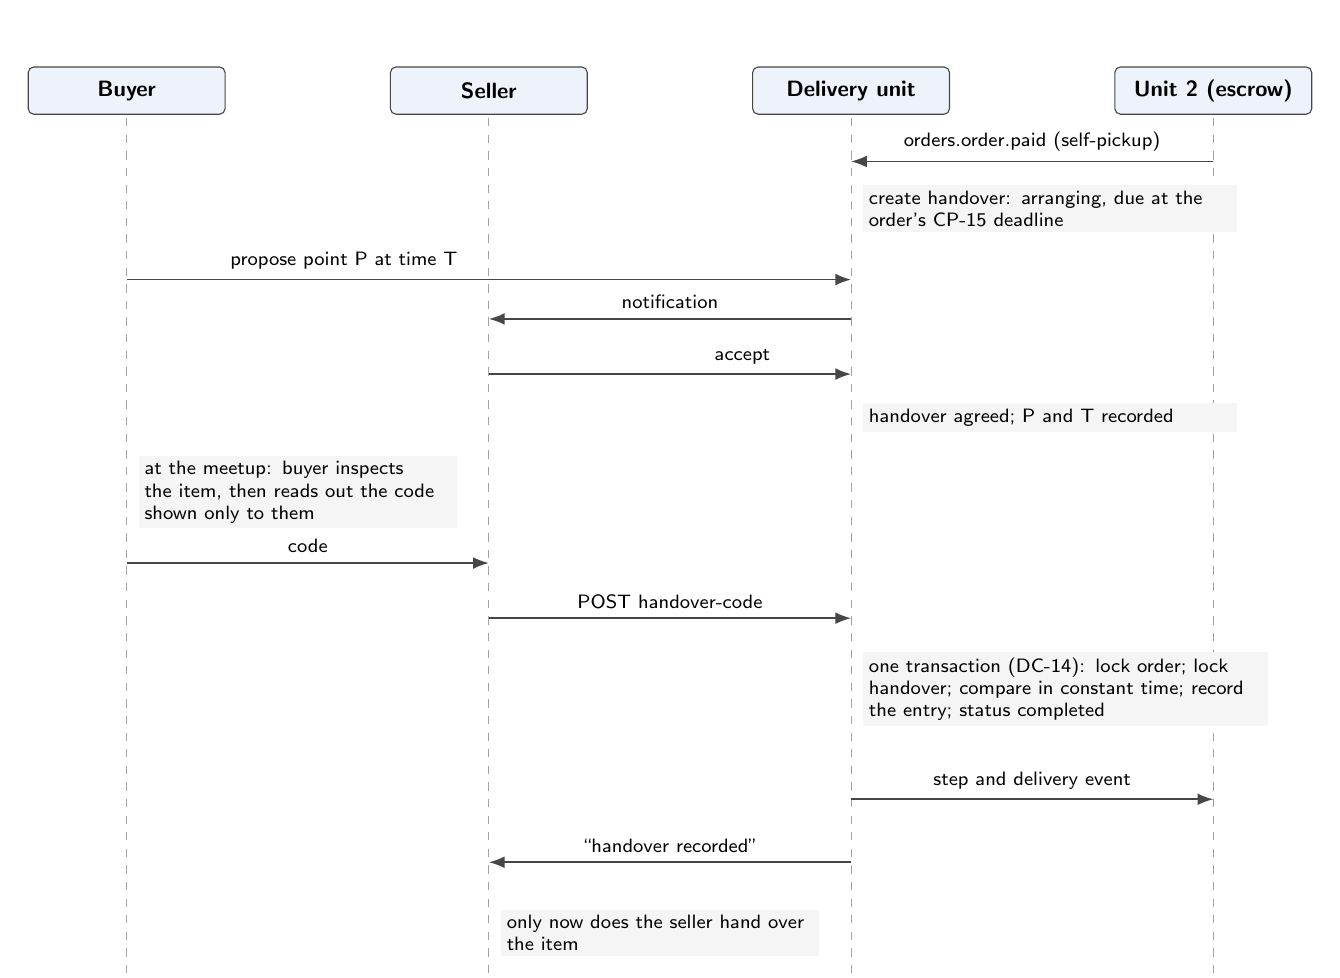
\begin{tikzpicture}[font=\sffamily\footnotesize,
  actor/.style={draw=edge, fill=boxb, rounded corners=2pt, minimum width=2.5cm, minimum height=0.6cm, font=\sffamily\footnotesize\bfseries},
  msg/.style={-{Latex[length=2mm]}, draw=edge, semithick},
  note/.style={font=\sffamily\scriptsize, align=left, text width=4.6cm, anchor=west, fill=boxd, inner sep=2pt}]
\def\B{0} \def\S{4.6} \def\A{9.2} \def\E{13.8}
\foreach \x/\t in {\B/Buyer, \S/Seller, \A/Delivery unit, \E/Unit 2 (escrow)}{
  \node[actor] at (\x,0) {\t};
  \draw[edge!50, dashed] (\x,-0.35) -- (\x,-11.4);}
\draw[msg] (\E,-0.9) -- node[above, font=\sffamily\scriptsize]{orders.order.paid (self-pickup)} (\A,-0.9);
\node[note] at (\A+0.15,-1.5) {create handover: arranging, due at the order's CP-15 deadline};
\draw[msg] (\B,-2.4) -- node[above, font=\sffamily\scriptsize, pos=0.3]{propose point P at time T} (\A,-2.4);
\draw[msg] (\A,-2.9) -- node[above, font=\sffamily\scriptsize]{notification} (\S,-2.9);
\draw[msg] (\S,-3.6) -- node[above, font=\sffamily\scriptsize, pos=0.7]{accept} (\A,-3.6);
\node[note] at (\A+0.15,-4.15) {handover agreed; P and T recorded};
\node[note, text width=3.9cm] at (\B+0.15,-5.1) {at the meetup: buyer inspects the item, then reads out the code shown only to them};
\draw[msg] (\B,-6.0) -- node[above, font=\sffamily\scriptsize]{code} (\S,-6.0);
\draw[msg] (\S,-6.7) -- node[above, font=\sffamily\scriptsize]{POST handover-code} (\A,-6.7);
\node[note, text width=5.0cm] at (\A+0.15,-7.6) {one transaction (DC-14): lock order; lock handover; compare in constant time; record the entry; status completed};
\draw[msg] (\A,-9.0) -- node[above, font=\sffamily\scriptsize]{step and delivery event} (\E,-9.0);
\draw[msg] (\A,-9.8) -- node[above, font=\sffamily\scriptsize]{``handover recorded''} (\S,-9.8);
\node[note, text width=3.9cm] at (\S+0.15,-10.7) {only now does the seller hand over the item};
\end{tikzpicture}}
\caption{Meetup handover (FR-DLV-04 to FR-DLV-06). The code entry and the escrow's delivery event commit together, or not at all.}
\label{fig:meetup-seq}
\end{figure}

\subsection{Suggesting a place}
The order view suggests the DV-27 (three) active curated points nearest the midpoint of the two parties' locations (FR-DLV-03). The points are police stations, shopping-mall entrances, bank branches and similar public places, maintained by an administrator. They are public, so their exact location is shown, with an ``open in maps'' link built from their coordinates.

The parties' own locations stay approximate (FR-DLV-07), and the midpoint needs care. A party who knew their own location and the exact midpoint could compute the other's location as twice the midpoint minus their own. Each location is therefore snapped to a coarse grid of DV-27 (0.02 degrees, about 2~km) before the midpoint is taken. The API returns only the points and their distance from the caller, never the midpoint or distances from it. The test moves one party by about 300~m and confirms that the suggestions and their order do not change.

\subsection{Agreeing a time}
Either party proposes a point and a time; the other accepts or declines (FR-DLV-04). The rules, enforced in \texttt{delivery.propose\_meetup} and \texttt{respond\_meetup}, are:
\begin{itemize}[nosep]
  \item only the buyer and the seller can propose, and only the other party can answer;
  \item the time must be at least DV-26 (1~hour) ahead, and at least DV-26 (2~hours) before the handover deadline, so that a meeting cannot be planned that the deadline would cut short;
  \item a new proposal from either side replaces the open one, so there is never more than one open proposal (tested with 20 simultaneous proposals: one open, 19 superseded);
  \item a proposal cannot be edited, only replaced;
  \item a proposal whose time has passed lapses instead of being accepted;
  \item rescheduling keeps the existing agreement in force until the new time is accepted.
\end{itemize}
Proposals outside daylight hours are allowed, but the order view shows a safety notice. Agreement is not required for the handover itself: what proves the handover is the code, not the plan.

\subsection{The handover code}
\label{sec:code}
\paragraph{What the parties see.} The buyer's order view shows a 6-digit code with the instruction: \emph{``Give this code to the seller only after you have inspected the item. Giving the code confirms that you have received it.''} The seller's view shows an entry box and the instruction: \emph{``Hand over the item only after this page shows Handover recorded.''} The second instruction protects the seller from a buyer who takes the item and walks away during a slow network request.

\paragraph{Derivation, not storage.} The code is never stored. It is computed on each request as
\[ \mathit{code} = \mathrm{HMAC\text{-}SHA\text{-}256}(\mathit{HANDOVER\_KEY},\ \mathit{orderId} \,\|\, \texttt{:} \,\|\, \mathit{codeVersion}) \bmod 10^6, \]
taking the first 8 bytes of the MAC as an unsigned integer, padded to 6 digits (DV-28). The reduction modulo $10^6$ makes some codes more likely than others by a relative amount below $10^{-13}$, which is negligible. Deriving the code has three benefits:
\begin{itemize}[nosep]
  \item a copy of the database reveals no codes;
  \item the buyer can reload the page and always see the same code;
  \item issuing a new code is just incrementing \texttt{code\_version}.
\end{itemize}
\texttt{HANDOVER\_KEY} is a new secret in Unit~1's key table (I-24). It is rotated only on compromise; a rotation changes every outstanding code, and both parties of each open handover are told to reload.

\paragraph{Checking an entry.} The service derives the expected code and compares it with the entry in constant time, then calls \texttt{delivery.record\_code\_entry} with the result, inside the DC-14 transaction. The function:
\begin{itemize}[nosep]
  \item locks the handover;
  \item refuses anyone but the seller, a locked or closed handover, and any entry after the deadline;
  \item logs the entry with its code version;
  \item on a correct entry, completes the handover;
  \item on a wrong entry, increments the count, and at CP-45 (5) locks code entry, opens a \texttt{code\_locked} issue and notifies both parties.
\end{itemize}
On a correct entry the service records the fulfilment step (\texttt{meetup\_handover}) and the delivery event (source \texttt{handover\_code}) through \texttt{EscrowCommands} in the same transaction, so the escrow's dispute window and auto-release time start at that moment (FR-PAY-07, FR-PAY-08).

\paragraph{Guessing.} With 5 attempts at a 6-digit code, the chance of guessing it is $5 / 10^6$. The limit holds under concurrency: 20 simultaneous wrong entries produced exactly 4 ``wrong'', 1 ``locked'' and 15 refusals, with 5 entries logged. Ten simultaneous correct entries produced one handover and nine refusals. Code entry is also rate-limited per seller (DV-28: 10 per minute), and a wrong code's response is the same whatever was entered.

\paragraph{Unlock.} A locked code stays locked until an operator, having contacted both parties, unlocks it with a reason (audited). Unlocking issues the next code version and resets the count; the old code no longer works. If nobody resolves the lock, the CP-15 deadline refunds the buyer as usual.

\paragraph{Secrecy.} The code is never written to logs, analytics, URLs or notifications (SEC-DAT-07), and in particular not to a push notification that could appear on a locked screen. It is returned only to the buyer, and only over the authenticated API.

\begin{figure}[!htbp]
\centering
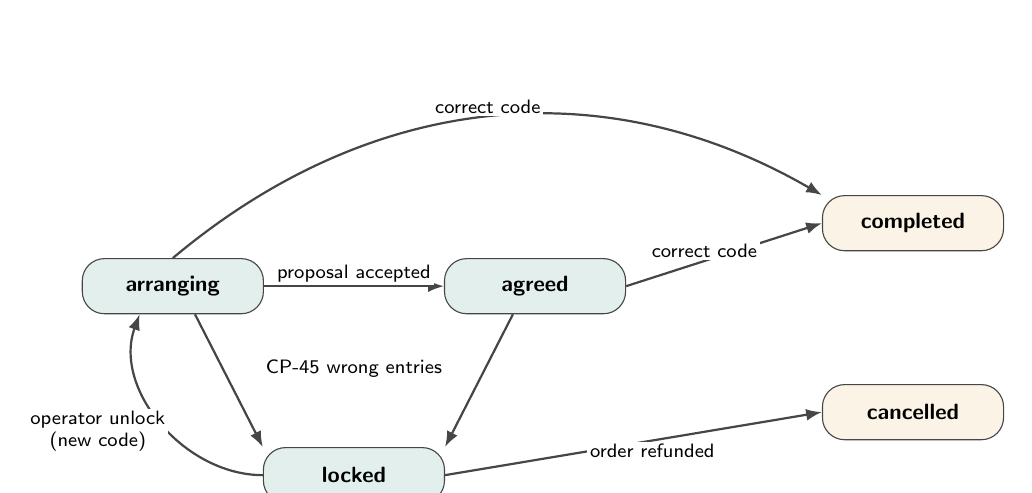
\begin{tikzpicture}[font=\sffamily\footnotesize,
  st/.style={draw=edge, rounded corners=8pt, fill=boxa, minimum width=2.3cm, minimum height=0.7cm, font=\sffamily\footnotesize\bfseries},
  tst/.style={st, fill=boxc},
  tr/.style={-{Latex[length=2mm]}, draw=edge, thick},
  lb/.style={font=\sffamily\scriptsize, align=center, fill=white, inner sep=1pt}]
\node[st] (a) at (0,0) {arranging};
\node[st] (g) at (4.6,0) {agreed};
\node[st] (l) at (2.3,-2.4) {locked};
\node[tst] (c) at (9.4,0.8) {completed};
\node[tst] (x) at (9.4,-1.6) {cancelled};
\draw[tr] (a) -- node[lb, above]{proposal accepted} (g);
\draw[tr] (g.east) -- node[lb, above, pos=0.4]{correct code} (c.west);
\draw[tr] (a.north) to[out=40, in=150] node[lb, above]{correct code} (c.north west);
\draw[tr] ([xshift=8pt]a.south) -- (l.north west);
\draw[tr] ([xshift=-8pt]g.south) -- (l.north east);
\node[lb] at (2.3,-1.05) {CP-45 wrong entries};
\draw[tr] (l.east) -- node[lb, below, pos=0.55]{order refunded} (x.west);
\draw[tr] (l.west) to[out=180, in=250] node[lb, left, pos=0.45]{operator unlock\\(new code)} ([xshift=-12pt]a.south);
\end{tikzpicture}
\caption{Handover status. Terminal states are shaded. An unlock returns to \texttt{agreed} if an agreement exists, otherwise to \texttt{arranging}. \texttt{arranging} and \texttt{agreed} also go to \texttt{cancelled} when the order is refunded (not drawn). The trigger \texttt{handover\_guard} refuses every other change.}
\label{fig:handover-states}
\end{figure}

\subsection{Deadline}
The deadline is Unit~2's \texttt{fulfilment\_due\_at}, copied to the handover when it is created. A code entered at or after it is refused. Unit~2's fulfilment job then refunds the buyer in full (FR-PAY-08), and this unit cancels the handover when it receives \texttt{orders.escrow.refunded}. Because both the code entry and the job lock the order first (DC-14), an entry just before the deadline is either recorded before the job runs, or refused after it; it can never be recorded for an order that has been refunded.

% ------------------------------------------------------------------
\section{Courier Delivery}
\label{sec:courier}

\subsection{Addresses}
\label{sec:addresses}
Exact addresses are Confidential data (SRS Section~7). A saved address keeps only its label and area in clear. The street lines, the contact name and any landmark are encrypted by Unit~1's \texttt{IdentityCrypto} with AES-256-GCM, with the table, column and row id as associated data. Copying a ciphertext into another row therefore fails to decrypt, so a shipment takes a copy re-encrypted under its own row id. The rules are:
\begin{itemize}[nosep]
  \item each party sees only their own address (FR-DLV-07); the other party sees the district;
  \item the courier receives both addresses and the parties' verified mobile numbers, over TLS, at booking, and nothing else (FR-PRV-01 names couriers as recipients);
  \item staff see addresses masked; showing one in full needs a reason and is logged (SEC-ACC-05);
  \item a shipment's addresses are erased DV-30 after the order closes (30~days, or 30~days after a cancelled shipment is final), unless a dispute is open; the database refuses to erase them from a shipment that is not final.
\end{itemize}

\subsection{Booking}
\label{sec:booking}
On \texttt{orders.order.paid} for a courier order, the service creates the forward shipment in \texttt{preparing}, with the claimed quote, the fee, the buyer's drop-off address, and the CP-16 pickup deadline copied from the order. The booking worker then:
\begin{enumerate}[nosep]
  \item waits for the seller's pickup address if none is saved, and notifies the seller (the pickup deadline still runs from payment, and the listing form warns sellers about this);
  \item calls \texttt{CourierPort.book} with the shipment id as the merchant reference, no cash to collect, and the billed weight and size;
  \item on success, stores the consignment id and moves the shipment to \texttt{booked};
  \item on failure, retries with exponential backoff and jitter (DV-29: from 1~minute, doubling to at most 1~hour, 8 attempts), then opens a \texttt{booking\_failed} issue.
\end{enumerate}
While the provider is failing, a circuit breaker makes new courier quotes return \texttt{503 courier\_unavailable}, so new courier checkouts are refused with a clear message. Existing shipments keep retrying (NFR-REL-04).

\subsection{Shipment status}
\begin{figure}[!htbp]
\centering
\resizebox{\textwidth}{!}{%
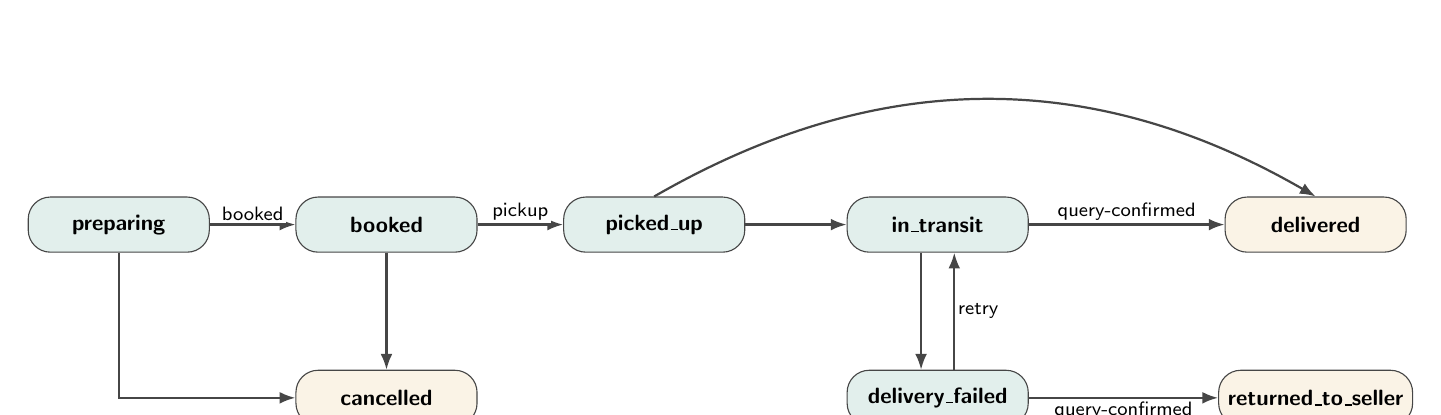
\begin{tikzpicture}[font=\sffamily\footnotesize,
  st/.style={draw=edge, rounded corners=8pt, fill=boxa, minimum width=2.3cm, minimum height=0.7cm, font=\sffamily\footnotesize\bfseries},
  tst/.style={st, fill=boxc},
  tr/.style={-{Latex[length=2mm]}, draw=edge, thick},
  lb/.style={font=\sffamily\scriptsize, align=center, fill=white, inner sep=1pt}]
\node[st] (p) at (0,0) {preparing};
\node[st] (b) at (3.4,0) {booked};
\node[st] (u) at (6.8,0) {picked\_up};
\node[st] (t) at (10.4,0) {in\_transit};
\node[st] (f) at (10.4,-2.2) {delivery\_failed};
\node[tst] (d) at (15.2,0) {delivered};
\node[tst] (r) at (15.2,-2.2) {returned\_to\_seller};
\node[tst] (c) at (3.4,-2.2) {cancelled};
\draw[tr] (p) -- node[lb, above]{booked} (b);
\draw[tr] (b) -- node[lb, above]{pickup} (u);
\draw[tr] (u) -- (t);
\draw[tr] (t) -- node[lb, above]{query-confirmed} (d);
\draw[tr] ([xshift=-6pt]t.south) -- ([xshift=-6pt]f.north);
\draw[tr] ([xshift=6pt]f.north) -- node[lb, right]{retry} ([xshift=6pt]t.south);
\draw[tr] (f) -- node[lb, below]{query-confirmed} (r);
\draw[tr] (u.north) to[out=30, in=150] (d.north);
\draw[tr] (p.south) |- (c.west);
\draw[tr] (b) -- (c);
\end{tikzpicture}}
\caption{Shipment status (FR-DLV-10). Terminal states are shaded. Not drawn: \texttt{picked\_up} and \texttt{in\_transit} may also go straight to \texttt{delivery\_failed} or \texttt{returned\_to\_seller}, and \texttt{delivery\_failed} to \texttt{delivered}. The trigger \texttt{shipment\_guard} refuses every other change.}
\label{fig:shipment-states}
\end{figure}

\subsection{Applying courier status reports}
\label{sec:status}
Courier reports arrive by webhook, by the reconciliation query (Section~\ref{sec:jobs}), and, before a missed-pickup refund, by \texttt{syncPickup}. They can arrive twice, late or out of order. Each one is handled in four steps:
\begin{enumerate}[nosep]
  \item \textbf{Authenticate.} The webhook endpoint verifies the provider's signature with the current environment's secret and rejects a timestamp outside CP-32 (5~minutes) (SEC-PAY-03, SEC-PAY-04, IF-COM-03). The mock courier signs its webhooks the same way, so the same code path is tested.
  \item \textbf{Confirm money-moving statuses.} \texttt{delivered} and \texttt{returned\_to\_seller} move money, so a webhook reporting them is treated as a hint. The service queries the provider's status API and applies only what the query returns. This is the courier equivalent of FR-PAY-02. The database enforces it: these two statuses are accepted only with source \texttt{provider\_query}.
  \item \textbf{Apply once.} \texttt{delivery.apply\_status} locks the shipment and records the provider's event id. A repeated id has no effect (\texttt{duplicate}). A report of an earlier stage, such as a pickup arriving after ``in transit'', changes nothing (\texttt{stale}). A report that skips \texttt{picked\_up}, such as \texttt{delivered} straight after \texttt{booked}, implies the pickup at the same time. A report that makes no sense, such as progress on a cancelled booking, is refused and opens a \texttt{status\_refused} issue. The provider's time is used, but never later than the server's clock and never earlier than the booking.
  \item \textbf{Act on the result} (forward shipments), in the same DC-14 transaction:
  \begin{itemize}[nosep]
    \item a pickup by the deadline calls \texttt{recordFulfilmentStep(courier\_pickup, at)};
    \item \texttt{delivered} calls \texttt{recordDeliveryEvent(courier\_delivered, at)}; this is the delivery event (FR-DLV-10);
    \item \texttt{returned\_to\_seller} calls \texttt{refundCourierReturned(charge)}, which refunds the buyer in full, including the fee, and books the courier's charge as a platform cost (FR-DLV-12).
  \end{itemize}
\end{enumerate}
A storm of 15 simultaneous reports (one event delivered 10 times, plus 5 other pickup events) produced exactly one applied pickup, 9 duplicates and 5 stale reports, and one history row.

\subsection{Pickup deadline}
If the courier has not picked up within CP-16 (3~days after payment), Unit~2's fulfilment job refunds the buyer in full (FR-DLV-11, FR-PAY-08). Webhooks can be delayed, so before refunding a courier order the job calls \texttt{DeliveryPort.syncPickup}. This queries the provider (with a DV-32 timeout of 10~seconds), outside any lock, and applies the result. A pickup that happened in time but was reported late is therefore counted. A pickup that happened after the deadline is recorded on the shipment but reported as late (\texttt{pickup\_on\_time} is false), so the escrow step is not recorded and the refund goes ahead. The parcel then follows the cancellation path below.

\subsection{Cancellation}
\label{sec:cancel}
When an order is refunded before its delivery event (cancellation under FR-PAY-09, or a missed deadline), the service stores \texttt{order\_cancelled\_at} on the shipment and:
\begin{itemize}[nosep]
  \item cancels a \texttt{preparing} shipment directly;
  \item asks the provider to cancel a \texttt{booked} one, and applies the confirmed cancellation;
  \item if the courier already has the parcel, requests a return to the seller. When the return is reported, no second refund is made; the courier's charge is booked as a platform cost through \texttt{recordCourierCost} (I-21).
\end{itemize}
A pickup reported after the order was cancelled is recorded, flagged \texttt{after\_cancel}, and raises a \texttt{pickup\_after\_cancel} issue, so that an operator makes sure the parcel goes back.

\subsection{Failed delivery, return and non-delivery}
\begin{itemize}[nosep]
  \item \textbf{Failed attempt.} \texttt{delivery\_failed} counts the attempt and notifies both parties. The courier may try again (back to \texttt{in\_transit}).
  \item \textbf{Return.} If the courier returns the item to the seller, the order is cancelled and the buyer refunded in full, including the delivery fee (FR-DLV-12). The SRS refunds the buyer in full even when the buyer refused the parcel. Repeated returns for one buyer are visible to Trust \& Safety (Unit~7) in the fulfilment records, because each costs the platform the courier's charge.
  \item \textbf{Not received.} Once CP-17 (7~days) has passed since pickup without delivery, \texttt{DeliveryQueries.notReceivedAllowed} becomes true and the buyer may open a \texttt{not\_received} dispute (FR-DLV-11, FR-DSP-01). Unit~2 raises its stalled-delivery review at CP-17 $+$ CP-18 if nobody does.
\end{itemize}

\subsection{Return shipments}
When a dispute is decided with ``refund after return'' (FR-DSP-06(d)), Unit~7 calls \texttt{quoteReturn} and \texttt{bookReturn}. The return is a second shipment for the same order, in the \texttt{return} direction, from the buyer to the seller, priced from the same fare table. The decision records who pays the return fare. When the return is delivered, or the seller confirms receipt, \texttt{delivery.return.delivered} tells Unit~7 to complete the refund.

\subsection{The mock courier}
\label{sec:mock}
Pathao and Steadfast sandbox access is not yet confirmed, so the mock courier is the default (C-3, SRS open issue). It is a module inside the backend that implements the provider side of \texttt{CourierPort}:
\begin{itemize}[nosep]
  \item a booking API that returns consignment ids like \texttt{MOCK-} followed by random characters, and honours the merchant reference, so it is idempotent;
  \item a status API;
  \item signed webhooks sent to the normal webhook endpoint;
  \item a simulator page for demonstrations, where an operator moves a parcel through pickup, transit, a failed attempt, delivery or return, with an optional return charge. Optionally, parcels advance automatically after configurable delays.
\end{itemize}
Every mock shipment is \texttt{simulated} (enforced by a database constraint). The order view, tracking page, notifications and documentation all state that the courier booking is simulated (FR-DLV-14, NFR-CMP-05). The module and its endpoints exist only in sandbox builds.

\subsection{Operator issues}
\label{sec:issues}
\begin{dtable}{@{}>{\ttfamily}p{3.6cm}>{\raggedright\arraybackslash}p{11.6cm}@{}}
\toprule
\textnormal{\textbf{Issue}} & \textbf{Raised when, and what the operator does} \\ \midrule \endhead
code\_locked & CP-45 wrong code entries. The operator contacts both parties, then unlocks or lets the deadline refund. \\
booking\_failed & The booking still fails after DV-29. The operator books manually with the provider, or cancels the order (full refund). \\
pickup\_after\_cancel & The courier took a parcel for a refunded order. The operator ensures the return. \\
status\_refused & A courier report the rules cannot place. The operator checks with the provider. \\
return\_failed & A return shipment fails. The operator arranges the return with both parties. \\
\bottomrule
\end{dtable}
\section{Scheduled Jobs}
\label{sec:jobs}
Each job scans only due rows through a partial index, and is safe to run on several instances at once (\texttt{FOR UPDATE SKIP LOCKED}), as in Units~2 and~3 (NFR-REL-03).
\begin{dtable}{@{}>{\raggedright\arraybackslash}p{3.6cm}>{\raggedright\arraybackslash}p{1.8cm}>{\raggedright\arraybackslash}p{9.8cm}@{}}
\toprule
\textbf{Job} & \textbf{Every} & \textbf{Action} \\ \midrule \endhead
Booking & 1 min & Book \texttt{preparing} shipments that are due, with backoff (DV-29). \\
Status reconciliation & 30 min & Query the provider for shipments in flight with no report for 6~hours, and apply the answer (DV-31). This catches lost webhooks, as FR-PAY-15 does for payments. \\
Proposal lapse & 15 min & Mark open proposals whose time has passed as \texttt{lapsed}. \\
Address erasure & daily & Erase shipment addresses after DV-30. \\
Provider events & daily & Delete event ids older than CP-32 (30~days). \\
\bottomrule
\end{dtable}
Deadline reminders for the meetup handover and the courier pickup (FR-NTF-07) are sent by Unit~6 from the deadlines this unit publishes; the refund at the deadline is Unit~2's job.

\section{Security and Privacy}
\begin{itemize}[nosep]
  \item \textbf{Authorisation.} Each endpoint names its party: buyer, seller or ``the other party'' for proposals; the seller alone enters the code; the buyer alone sees it. The database functions check the same parties again, so a service bug cannot let a third person propose, answer or enter a code (tested). Staff actions are limited to those listed in the API, each with a reason, and audited (SEC-ACC-01 to SEC-ACC-03).
  \item \textbf{The handover code} is derived, never stored, never logged, and returned only to the buyer. Entry is limited to CP-45 wrong attempts, then locked; it is also rate-limited (Section~\ref{sec:code}).
  \item \textbf{Location privacy.} Parties see each other's district only. Meetup suggestions use snapped locations, and the midpoint is never returned. Distances are whole kilometres from rounded coordinates (FR-DLV-07).
  \item \textbf{Addresses} are encrypted field by field, shown only to their owner and the courier, masked for staff, and erased on schedule (Section~\ref{sec:addresses}).
  \item \textbf{Courier integration.} Webhooks are signed, time-limited and idempotent. Money-moving statuses are confirmed by a status query. Booking is idempotent. Credentials are separate per environment, and provider endpoints are fixed (SEC-PAY-03 to SEC-PAY-05, SEC-PAY-07, SEC-INP-05).
  \item \textbf{Integrity.} Code entries, shipment history and fare tables are append-only, and the application role cannot update them or delete shipments (tested). Quotes cannot be changed once issued.
  \item \textbf{Abuse limits.} Quotes are limited to 30 per hour per user (DV-23), and code entry to 10 per minute per seller (DV-28) (SEC-ABU-01).
\end{itemize}

\subsection{Threats considered}
\begin{dtable}{@{}>{\raggedright\arraybackslash}p{4.6cm}>{\raggedright\arraybackslash}p{10.6cm}@{}}
\toprule
\textbf{Threat} & \textbf{Defence} \\ \midrule \endhead
Seller records a handover without meeting & Needs the buyer's code: at most 5 guesses at 6 digits, then locked. \\
Buyer takes the item without giving the code & The seller is told to hand over only after ``Handover recorded'' appears. \\
Buyer pressed to give the code before inspecting & The instruction says what the code means; a dispute remains possible within CP-18 for \texttt{not\_as\_described} or \texttt{damaged}. \\
Location stalking through meetup suggestions & Snapped locations; no midpoint in the API; district only. \\
Forged or replayed courier webhook & Signature, timestamp tolerance, event-id store; delivery and return confirmed by query. \\
Courier collects cash at the door & Bookings always set no cash to collect; the order view says the item is paid for. \\
Fee manipulation & The fee comes only from a server-issued quote, fixed and claimed once; client amounts are ignored (SEC-PAY-06). \\
\bottomrule
\end{dtable}

\section{Parameters}
\textbf{SRS parameters used:} CP-14 (self-pickup threshold); CP-15 and CP-16 (handover and pickup deadlines, read from the order); CP-17 (non-delivery dispute); CP-26 (delivery margin, applied by Unit~2); CP-32 (webhook tolerance and event retention); CP-35 (rate limits); CP-43 (fare table); CP-45 (wrong code entries).

\textbf{Design values introduced} (continuing DV-1 to DV-22):
\begin{dtable}{@{}>{\bfseries}p{1.3cm}>{\raggedright\arraybackslash}p{5.0cm}>{\raggedright\arraybackslash}p{3.6cm}>{\raggedright\arraybackslash}p{5.0cm}@{}}
\toprule
\textnormal{\textbf{ID}} & \textbf{Value} & \textbf{Default} & \textbf{Reason} \\ \midrule \endhead
DV-23 & Quote validity; quote rate limit & 30 minutes; 30 quotes per hour per user & Longer than the CP-13 checkout hold. \\
DV-24 & Largest billed weight by courier & 10 kg & Rate cards cap parcel weight; lower it if the provider's limit is lower (Paperfly's is 8~kg). \\
DV-25 & Minimum billed weight by size class & small 0, medium 2~kg, large 5~kg; oversize not by courier & Couriers charge bulky parcels by volume. \\
DV-26 & Meetup time window & at least 1~h ahead, at least 2~h before the deadline & No meeting the deadline cuts short. \\
DV-27 & Meetup suggestions & 3 points; locations snapped to 0.02$^\circ$ & Choice without revealing locations. \\
DV-28 & Handover code & 6 digits, HMAC-SHA-256 derivation; entry 10 per minute per seller & As OTPs (SEC-AUTH-09); never stored. \\
DV-29 & Booking retries & from 1~min, doubling to 1~h; 8 attempts & Then an operator issue. \\
DV-30 & Shipment address retention & 30 days after the order closes, unless a dispute is open & Long enough for a late dispute; then erased. \\
DV-31 & Courier status reconciliation & every 30 min, shipments silent for 6~h & Catches lost webhooks. \\
DV-32 & Pickup query before a missed-pickup refund & 10-second timeout & A late webhook does not cost the seller the sale. \\
\bottomrule
\end{dtable}

\section{Testing}
\label{sec:testing}
\begin{dtable}{@{}>{\raggedright\arraybackslash}p{3.2cm}>{\raggedright\arraybackslash}p{12cm}@{}}
\toprule
\textbf{Level} & \textbf{Cases} \\ \midrule \endhead
Database (done) & 93 checks in \texttt{04\_delivery\_tests.sql}, each rejection required to fail on its intended rule. They cover zones, billed weight, fares and fare versions; the 2~km recommendation boundary; quotes, addresses, claiming and expiry; meetup suggestions and snapping; proposals, counter-proposals, rescheduling and lapse; the handover code, the lock and the unlock; the deadline; shipments, their quote and addresses; duplicates, stale and implied statuses, query confirmation, late pickup, clock clamping, return charge, cancellation and refusals; non-delivery eligibility; return shipments; issues; and grants. The Unit~1 to~3 scripts still pass with this schema loaded. \\
Concurrency (done) & Five races, three runs each on fresh databases, with the same counts every time: 20 wrong codes (4 wrong, 1 lock, 15 refused); 10 correct codes (1 accepted); 20 proposals (1 open); 15 courier reports (1 applied); 10 claims of one quote (1 claimed). See Appendix~\ref{app:tests}. \\
Unit & Code derivation (fixed vectors, 6 digits, leading zeros); constant-time comparison; snapping; the webhook signature and timestamp checks; the circuit breaker; the indicative fee equals the quoted fee. \\
Integration & Handover plus escrow is atomic (an escrow error rolls back the code entry). A deadline race between a code entry and Unit~2's job. Mock courier end to end: book, pickup, transit, failed attempt, delivered, with the escrow's delivery event; return to seller with a charge; cancellation before and after pickup. \texttt{syncPickup} counts a late-reported pickup. \\
Security & Negative authorisation tests for every endpoint (SEC-SDL-09). The seller's responses never contain the code. Logs contain no code or address (checked by a log scan in CI). \\
\bottomrule
\end{dtable}

\section{Notes for Integration}
\label{sec:notes}
\begin{enumerate}[label=\textbf{I-\arabic*}, leftmargin=*, nosep]
  \setcounter{enumi}{18}
  \item \textbf{Unit 2: \texttt{orders.order.paid} payload.} It must carry the fulfilment method, buyer, seller, \texttt{fulfilment\_due\_at} and the delivery quote id.
  \item \textbf{Unit 2: \texttt{OrdersPort.lockForFulfilment(orderId, tx)}.} New. Locks the order row and returns its status, fulfilment, parties, deadline and whether the step or delivery event is recorded (DC-14).
  \item \textbf{Unit 2: quotes and courier costs.} \texttt{DeliveryPort.getQuote} becomes \texttt{claimQuote}, which also checks quantity and allows one use. New \texttt{EscrowCommands.recordCourierCost(orderId, amount, tx)} books a return charge for an order that was already refunded.
  \item \textbf{Unit 2: fulfilment job.} Before refunding a courier order for a missed pickup, it calls \texttt{DeliveryPort.syncPickup} outside its lock. \texttt{recordFulfilmentStep} is called only for a pickup made by the deadline.
  \item \textbf{Unit 3.} New \texttt{ListingsQueries.fulfilmentFacts(listingId)}. The listing form, and a constraint added to \texttt{listings.listings}, should refuse courier options for the \texttt{over\_10kg} weight class and the \texttt{oversize} size class, which no fare covers (DV-24, DV-25).
  \item \textbf{Unit 1.} New \texttt{IdentityQuery.getApproxArea(userId)}. Add \texttt{HANDOVER\_KEY} and the courier API and webhook secrets to the key table (Unit~1 Section~3).
  \item \textbf{Unit 6} delivers the meetup, handover, lock and shipment notifications, and the deadline reminders (FR-NTF-07). No notification may contain the handover code.
  \item \textbf{Unit 7} hosts the delivery issue queue and the unlock action. It uses \texttt{fulfilmentRecord} in the case file (FR-DSP-05), \texttt{notReceivedAllowed} for \texttt{not\_received} disputes, and \texttt{quoteReturn} and \texttt{bookReturn} for outcome (d).
  \item \textbf{Unit 8} (frontend) shows the code screen with its instruction, the seller's entry screen with the ``hand over only after'' instruction, a ``simulated'' banner on every mock shipment, and map links for meetup points only.
  \item \textbf{SRS clarifications proposed:}
  \begin{itemize}[nosep]
    \item FR-DLV-08: distance enters the fare through the zone, as in the cited rate cards;
    \item FR-DLV-10: add the internal statuses \texttt{preparing} and \texttt{cancelled}, and state that \texttt{delivered} is confirmed by a status query;
    \item FR-DLV-11: a pickup made after CP-16 does not count, and the parcel is returned;
    \item FR-LST-03 refers to FR-DLV-07 for the fare model; it should refer to FR-DLV-08;
    \item CP-43: name the rate card used for the seed values, and add DV-23 to DV-32 to the SRS parameter table.
  \end{itemize}
\end{enumerate}

\appendix
\section{Traceability}
\label{app:trace}
{\small\begin{longtable}{@{}>{\ttfamily}p{2.4cm}>{\raggedright\arraybackslash}p{10.6cm}>{\raggedright\arraybackslash}p{2.2cm}@{}}
\toprule \textnormal{\textbf{Requirement}} & \textbf{Design element} & \textbf{Section} \\ \midrule \endhead
FR-DLV-01 & Distance from rounded coordinates, shown in whole km & \ref{sec:pricing} \\
FR-DLV-02 & \texttt{recommended\_method}; buyer chooses among allowed methods; no fee for self-pickup & \ref{sec:pricing} \\
FR-DLV-03 & Curated \texttt{meetup\_points}; \texttt{suggest\_points} near the midpoint & \ref{sec:meetup} \\
FR-DLV-04 & \texttt{propose\_meetup}, \texttt{respond\_meetup}; one open proposal; agreed point on the handover & \ref{sec:meetup} \\
FR-DLV-05 & Handover only for paid orders; no cash option; courier bookings collect no cash & \ref{sec:meetup}, \ref{sec:courierport} \\
FR-DLV-06 & Derived code shown to the buyer only; \texttt{record\_code\_entry}; CP-45 lock; unlock & \ref{sec:code} \\
FR-DLV-07 & District only; snapped midpoint; encrypted addresses, own address only & \ref{sec:meetup}, \ref{sec:addresses} \\
FR-DLV-08 & Zones, billed weight, versioned fare table; quote fixed at checkout & \ref{sec:pricing} \\
FR-DLV-09 & One total; no courier choice for the buyer & \ref{sec:pricing} \\
FR-DLV-10 & Shipment status machine; query-confirmed delivery as the delivery event & \ref{sec:status} \\
FR-DLV-11 & Pickup deadline with \texttt{syncPickup}; \texttt{not\_received\_allowed} after CP-17 & \ref{sec:status}, \ref{sec:cancel} \\
FR-DLV-12 & Return to seller: full refund including fee; return charge as platform cost & \ref{sec:status}, \ref{sec:cancel} \\
FR-DLV-13 & Fee fixed on the order; split by Unit~2 & \ref{sec:pricing} \\
FR-DLV-14 & \texttt{simulated} on every mock shipment (constraint); labels & \ref{sec:mock} \\
FR-PAY-07 & Delivery event recorded only by code or query-confirmed delivery & \ref{sec:code}, \ref{sec:status} \\
FR-PAY-08 & Fulfilment step via DC-14; entry refused after the deadline & \ref{sec:dc14}, \ref{sec:code} \\
FR-PAY-09 & Handover and shipment cancelled on refund before delivery & \ref{sec:cancel} \\
FR-DSP-01 & \texttt{notReceivedAllowed} & \ref{sec:cancel} \\
FR-DSP-05 & \texttt{fulfilmentRecord}: proposals, code entries, shipments, history & \ref{sec:api} \\
FR-DSP-06 & Return shipments; \texttt{delivery.return.delivered} & \ref{sec:cancel} \\
FR-NTF-07 & Deadlines and events for reminders & \ref{sec:jobs} \\
FR-PRV-01 & Courier named as recipient of addresses and phone numbers & \ref{sec:addresses} \\
SEC-PAY-03 & Webhook signature check & \ref{sec:status} \\
SEC-PAY-04 & Timestamp tolerance; \texttt{provider\_events} & \ref{sec:status} \\
SEC-PAY-05 & Separate courier credentials per environment & \ref{sec:courierport} \\
SEC-PAY-06 & Fee only from a server-issued quote & \ref{sec:pricing} \\
SEC-PAY-07 & Shipment id as idempotent merchant reference & \ref{sec:courierport} \\
SEC-DAT-07 & Code and addresses never logged & \ref{sec:code} \\
SEC-ACC-05 & Masked addresses for staff; logged display & \ref{sec:addresses} \\
SEC-INP-05 & Fixed provider endpoints & \ref{sec:courierport} \\
SEC-ABU-01 & Quote and code-entry limits & \ref{sec:code} \\
IF-SW-04 & \texttt{CourierPort}; mock, Pathao and Steadfast adapters & \ref{sec:courierport} \\
IF-COM-03 & Dedicated webhook endpoint & \ref{sec:api} \\
NFR-REL-03 & Jobs on partial indexes, \texttt{SKIP LOCKED} & \ref{sec:jobs} \\
NFR-REL-04 & Circuit breaker refuses new courier checkouts & \ref{sec:booking} \\
NFR-CMP-05 & Simulated labels & \ref{sec:mock} \\
DR-06 & Proposals, code entries, shipments, shipment history & \ref{sec:data} \\
\bottomrule
\end{longtable}}

\section{Database Schema and Tests}
\label{app:ddl}
\subsection{Test results}
\label{app:tests}
Loaded after the Unit~1 to Unit~3 schemas in PostgreSQL 16, using PostgreSQL 15 features only. Every check passed. The concurrency results follow the script output.
{\scriptsize
\begin{verbatim}
PASS  CP-43 both ends inside Dhaka: inside zone
PASS  CP-43 inside Dhaka to a suburb: suburbs zone
PASS  CP-43 suburb to outside Dhaka: outside zone
PASS  a listing near Dhanmondi is inside Dhaka; near Savar (same district) is a suburb
PASS  a district with no listed areas is outside Dhaka
PASS  DV-25 billed weight: 1 kg small = 1; 1 kg large = 5 (volumetric); 3 x 2 kg = 6
PASS  DV-24 over 10 kg in total, an over-10 kg item or an oversize item cannot go by courier
PASS  fare v1: inside Dhaka 1 kg = BDT 50; 5 kg = 65 + 3 x 15 = BDT 110; outside 2 kg = BDT 120
PASS  a fare version is not used until it has all three zones
PASS  a complete newer version takes effect
PASS  fare rows are append-only (publish a new version instead) [append-only]
PASS  a fare must not fall with weight [fare_rises_with_weight]
PASS  a published fare version names the administrator [fare_version_has_creator]
PASS  FR-DLV-02 at or below CP-14 (2 km) self-pickup is recommended; above it, courier
PASS  FR-DLV-02 only allowed methods are recommended
PASS  FR-DLV-08 Dhanmondi to Mirpur, 1 kg: inside Dhaka, BDT 50, distance recorded
PASS  FR-DLV-08 Dhanmondi to Savar: suburbs, BDT 80
PASS  FR-DLV-08 Dhanmondi to Chattogram, 2 units: outside Dhaka, 2 kg, BDT 120
PASS  FR-DLV-02 no courier quote for a pickup-only listing [does not offer courier]
PASS  DV-24 no quote for a parcel over the courier limit [too heavy or too large]
PASS  FR-DLV-07 a quote uses the buyer's own drop-off address [buyer's own]
PASS  the drop-off address must lie in the quoted area [in the quoted area]
PASS  a checkout quote always has a drop-off address [checkout_quote_has_address]
PASS  FR-DLV-08 a quote is fixed once issued [fixed once issued]
PASS  a quote is claimed only by the buyer it was issued to [does not match]
PASS  a quote is claimed only for the quantity it priced [does not match]
PASS  FR-DLV-08 claiming fixes the fee on the order (BDT 50)
PASS  a quote is used by one order only [already used]
PASS  DV-23 an expired quote cannot be used [quote expired]
PASS  FR-DLV-03 suggestions are the nearest active points to the midpoint, in order
PASS  FR-DLV-07 the midpoint uses snapped locations: moving one party by 300 m does not change it
PASS  a handover starts as arranging [starts as arranging]
PASS  FR-DLV-04 only the buyer or the seller can propose a meetup [only the buyer or the seller]
PASS  DV-26 a meetup must be at least the lead time ahead [meetup time must be]
PASS  DV-26 a meetup must leave the buffer before the CP-15 deadline [meetup time must be]
PASS  FR-DLV-03 a meetup is only at an active curated point [not an active meetup point]
PASS  FR-DLV-04 a counter-proposal replaces the open one; only one is open
PASS  FR-DLV-04 the proposer cannot accept their own proposal [only the other party]
PASS  FR-DLV-04 the other party accepts; the agreed point and time are recorded
PASS  a proposal cannot be edited after it is made [cannot be edited]
PASS  rescheduling: the earlier agreement stands until the new time is accepted
PASS  rescheduling: accepting the new time supersedes the old agreement
PASS  an answered proposal cannot be answered again [no longer open]
PASS  a proposal whose time has passed lapses instead of being accepted
PASS  FR-DLV-06 only the seller enters the handover code [only the seller]
PASS  CP-45 must stay within its permitted range 3 to 10 [between 3 and 10]
PASS  FR-DLV-06 wrong entries 1 to 4 are counted
PASS  FR-DLV-06 the 5th wrong entry (CP-45) locks code entry, opens an issue and notifies both
PASS  FR-DLV-06 no entry is accepted while locked, not even the right code [code entry is locked]
PASS  the wrong-entry count cannot be reset by an ordinary update [change only by an unlock]
PASS  an operator unlock issues code version 2, resets the count and keeps the agreement
PASS  FR-DLV-06 the correct code records the handover (the delivery event)
PASS  after the handover no further code is accepted [handover is closed]
PASS  a completed handover cannot be reopened or cancelled [handover is closed]
PASS  DR-06 every entry is logged with its code version (5 wrong on v1, 1 right on v2)
PASS  the code-entry log is append-only [append-only]
PASS  FR-PAY-08 no handover is recorded after the CP-15 deadline [deadline has passed]
PASS  an order cancelled before handover cancels the handover
PASS  a shipment uses its own claimed quote and fee [own claimed quote and fee]
PASS  FR-DLV-14 a mock booking is always marked simulated [shipment_simulated_iff_mock]
PASS  one forward shipment per order [shipment_one_per_direction]
PASS  FR-DLV-07 a booking needs the seller's pickup address [shipment_addresses]
PASS  a booking needs the provider's consignment id [shipment_booked_fields]
PASS  the consignment id is fixed once booked [consignment id is fixed]
PASS  FR-DLV-10 pickup by webhook is applied, on time, and reported for the fulfilment step
PASS  SEC-PAY-04 the same provider event again has no effect
PASS  FR-DLV-10 in transit is applied
PASS  a late-arriving older status (picked up after in transit) is ignored as stale
PASS  FR-DLV-10 a webhook alone cannot record delivery [provider status query]
PASS  FR-DLV-10 delivery confirmed by status query is the delivery event
PASS  nothing changes a delivered shipment (a later failure report is stale)
PASS  a final shipment cannot be edited [shipment is final]
PASS  DR-06 the history records every status in order, with its source
PASS  DV-30 a final shipment's addresses can be erased
PASS  a delivery reported straight after booking implies the pickup, at the same time
PASS  FR-DLV-11 a pickup after the CP-16 deadline is recorded but reported as late
PASS  a provider time in the future is clamped to the server time
PASS  FR-DLV-12 return to seller (confirmed by query) records the courier's charge
PASS  a pickup after the order was cancelled is flagged and raises an operator issue
PASS  a provider-confirmed cancellation before pickup cancels the shipment
PASS  progress reported on a cancelled booking is refused and sent to an operator
PASS  a status that skips the booking (preparing to picked up) is refused
PASS  the courier's return charge is recorded only on a return [shipment_charge_only_on_return]
PASS  DV-30 addresses are erased only after the shipment is final [shipment_erase_only_when_final]
PASS  FR-DLV-11 a not_received dispute is allowed CP-17 (7 days) after pickup without delivery
PASS  FR-DLV-11 ... but not before
PASS  FR-DSP-06(d) a return quote is claimed for an order that already used a checkout quote
PASS  FR-DSP-06(d) the return's delivery is published for Disputes to complete the refund
PASS  an issue is resolved only with a staff member and a reason [issue_resolution]
PASS  DC-6 outbox events are named delivery.<entity>.<past> [outbox_event_type_check]
PASS  application role cannot rewrite shipment history [permission denied]
PASS  application role cannot delete shipments [permission denied]
PASS  SEC-PAY-04 the application purges event ids older than CP-32 (30 days), and only those

93 checks passed (04_delivery_tests.sql, PostgreSQL 16.15 with the Unit 1-3 schemas loaded). The
Unit 1-3 test scripts still pass with Unit 4 loaded (46, 45 and 67 checks).

Concurrency (04_delivery_concurrency.sh; sessions released together by an advisory lock).
Three runs on fresh databases gave the same counts; only the quote race's winner differed.
  Wrong-code race: 20 sessions enter a wrong code at once (CP-45 = 5)
    results: wrong 4, locked 1, refused as locked 15
    database: wrong_entries=5, status=locked, logged entries=5
  Correct-code race: 10 sessions enter the right code at once
    results: accepted 1, refused as closed 9
    database: completed events=1
  Proposal race: 20 sessions (buyer and seller alternately) propose at once
    results: created 20, errors 0
    database: open=1, superseded=19
  Webhook storm: the same pickup event delivered 10 times plus 5 other pickup events, at once
    results: applied 1, duplicate 9, stale 5
    database: picked_up history rows=1
  Quote race: 10 orders claim the same quote at once
    results: claimed 1, refused as used 9
    database: quote order=d0000000-0000-4000-8000-0000000000cd
\end{verbatim}
}
\subsection{Schema}
\lstinputlisting[language=SQLpg]{sql/04_delivery.sql}
\end{document}
